\chapter{Análise dos Resultados}
\label{ch:5resultados}

Este capítulo apresenta os resultados obtidos durante a execução dos experimentos comparativos entre os protocolos de comunicação \gls{rest}, \gls{grpc}~e Apache Thrift em um ambiente de microsserviços para assistentes virtuais multimodais no contexto financeiro. Foram conduzidos testes nos três cenários definidos no \autoref{ch:4metodologia}: Simples, Tradicional e Complexo, cada um submetido a uma carga constante de 1.000 usuários simultâneos. Para cada combinação de cenário e protocolo, foram coletadas \textbf{15 amostras}, totalizando \textbf{135 execuções}. 

A análise é realizada a partir de duas perspectivas principais: (1) a do cliente, utilizando métricas de latência (avg, max, p90, p95) e throughput coletadas pela ferramenta k6; e (2) do servidor, com métricas de uso de CPU e memória coletadas via Prometheus. Para validar estatisticamente as diferenças de desempenho observadas entre os protocolos e cenários, foi realizada uma Análise de Variância (ANOVA) fatorial de dois fatores para cada métrica de interesse, melhor visualizada na \autoref{tab:5-resultados-anova}. Esta análise confirmou que as diferenças de desempenho entre os protocolos são estatisticamente significativas (\(p < 0,05\)) em todos os cenários, validando a robustez das conclusões.

\begin{table}[h]
\centering
\caption{Resultados da ANOVA fatorial para as métricas de desempenho}
\label{tab:5-resultados-anova}
\begin{tabular}{lcccccc}
\hline
\textbf{Métrica} & \textbf{Efeito} & \textbf{Soma Quad}. & \textbf{gl} & \textbf{F} & \textbf{p-valor} & \textbf{$\eta^2$} \\ 
\hline
Latência & Cenário & 193,46 & 2 & 1762,54 & $< 0,001$ & 0,93 \\
(ms) & Protocolo & 2,02 & 2 & 18,37 &$< 0,001$ & 0,23 \\
& Interação & 1,05 & 4 & 4,79 & $< 0,001$ & 0,13 \\
\hline
Uso de CPU & Cenário & 223351,31 & 2 & 2177,70 & $< 0,001$ & 0,91 \\
(\%) & Protocolo & 12267,87 & 2 & 119,61 & $< 0,001$ & 0,49 \\
& Interação & 5069,15 & 4 & 24,71 & $< 0,001$ & 0,44 \\
\hline
Uso de Memória & Cenário & 20223080 & 2 & 3048,48 & $< 0,001$ & 0,93 \\
(MB) & Protocolo & 651911 & 2 & 98,27 & $< 0,001$ & 0,28 \\
& Interação & 165198 & 4 & 12,45 & $< 0,001$ & 0,28 \\
\hline
Throughput & Cenário & 202876500 & 2 & 6203,61 & $< 0,001$ & 0,97 \\
(req/s) & Protocolo & 6130671 & 2 & 187,47 & $< 0,001$ & 0,58 \\
& Interação & 10133020 & 4 & 154,93 & $< 0,001$ & 0,83 \\
\hline
\end{tabular}
{\par \raggedright \footnotesize Fonte: Elaborado pelo autor.}
\end{table}

A discussão está organizada por cenário de complexidade crescente, permitindo observar o comportamento dos protocolos sob diferentes condições de estresse.

\section{Cenário Simples}
\label{sec:cenario_simples}

Neste cenário, representa-se consultas diretas e objetivas ao assistente virtual, caracterizadas por baixa complexidade computacional e processamento mínimo pelo módulo de \acrfull{ia} generativa.

No cenário simples, observam-se diferenças significativas entre os protocolos, conforme ilustrado na \autoref{fig:5-res-simples} e detalhado na \autoref{tab:5-res-simples}. As latências médias apresentam uma gradação clara: 280\,ms para \gls{grpc}, 346\,ms para Thrift e 477\,ms para \gls{rest}. Esta distribuição reflete as características arquiteturais de cada protocolo: serialização binária versus textual e otimizações de transporte. O throughput segue padrão similar, com \gls{grpc} alcançando 3.563\,req/s, Thrift 2.891\,req/s e \gls{rest} 2.095\,req/s. Em termos de recursos, os protocolos binários demonstram eficiência superior: \gls{grpc} consome 13,1\% de CPU e 303\,MB de RAM, Thrift utiliza 14\% de CPU e 315\,MB de RAM, enquanto \gls{rest} demanda 18,1\% de CPU e 362\,MB de RAM, evidenciando o impacto da serialização \acrshort{json} mesmo em cargas simples.


\begin{figure}[H]
\caption{Resultados Comparativos - Cenário Simples}
    \label{fig:5-res-simples}
    \centering
    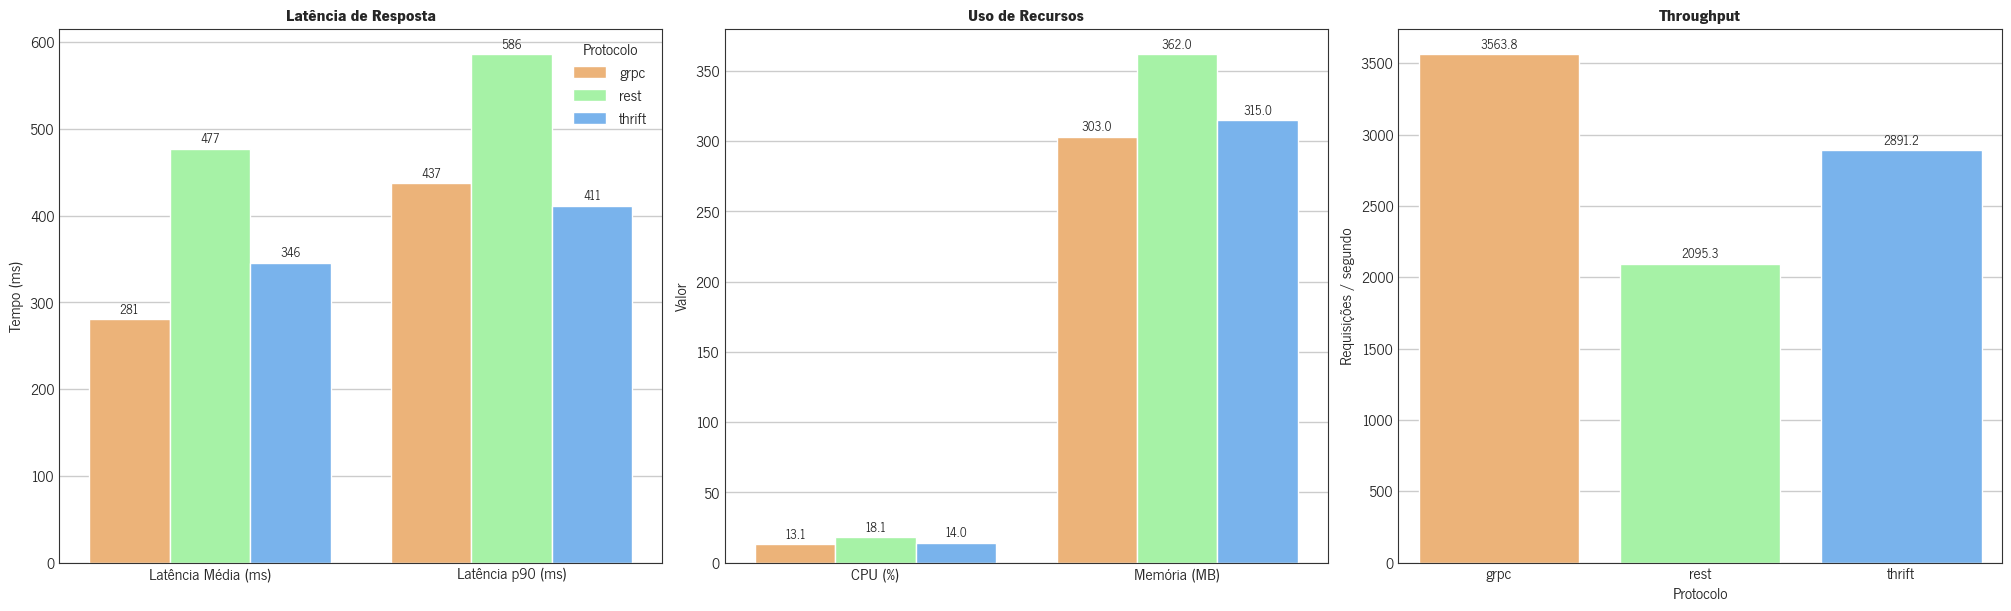
\includegraphics[width=1\linewidth]{imagens/resultados/5-resultados-simples.png}    
    {\par \raggedright \footnotesize Fonte: Elaborado pelo autor.\par}
\end{figure}

\begin{table}[H]
\centering
\caption{Métricas de desempenho e uso de recursos - Cenário Simples}
\label{tab:5-res-simples}
\begin{tabular}[\linewidth]{lrrrrrrr}
\hline
Protocolo & Avg (ms) & Max (ms) & p90 (ms) & p95 (ms) & Throughput (req/s) & CPU (\%) & \acrshort{ram} (MB) \\
\hline
\textbf{\acrshort{grpc}} & 280,60 & 536,43 & 437,34 & 500,18 & 3.563,80 & 13,10 & 303 \\
\textbf{Thrift} & 345,87 & 545,47 & 401,14 & 435,93 & 2.891,20 & 14,00 & 315 \\
\textbf{\gls{rest}} & 477,25 & 653,16 & 510,44 & 512,56 & 2.095,30 & 18,10 & 362 \\
\hline
\end{tabular}
{\par \raggedright \footnotesize Fonte: Elaborado pelo autor.\par}
\end{table}

\subsection{\acrshort{grpc}}

O protocolo \textbf{\acrshort{grpc}} apresentou o melhor desempenho geral no \emph{Cenário Simples}, conforme resumido na \autoref{tab:5-res-simples} e ilustrado na \autoref{fig:5-res-simples}. A \autoref{tab:5-res-simples-grpc} está organizada em colunas que descrevem:

\begin{itemize}
\item \textbf{Avg (ms)}: latência média de resposta;
\item \textbf{Max (ms)}: maior latência observada;
\item \textbf{p90 (ms)} e \textbf{p95 (ms)}: latências de cauda (percentis 90 e 95);
\item \textbf{Throughput (req/s)}: taxa média de requisições por segundo;
\item \textbf{CPU (\%)} e \textbf{\acrshort{ram} (MB)}: consumo médio de recursos.
\end{itemize}

Os valores destacados em \textcolor{green}{verde} correspondem ao melhor desempenho observado (menor latência, maior \emph{throughput} ou menor uso de recursos), enquanto os valores em \textcolor{red}{vermelho} indicam desempenho inferior em relação à métrica. Em número absoluto, apresentam-se os valores do protocolo atual, e nas demais linhas constam as variações $\Delta$~em comparação.

\newcommand{\superior}[1]{\cellcolor{green!12}{#1}}
\newcommand{\inferior}[1]{\cellcolor{red!12}{#1}}

\begin{table}[H]
\centering
\caption{\gls{grpc} comparado com os demais protocolos — Cenário Simples (Thrift/\gls{rest} em $\Delta$\% vs \gls{grpc})}
\label{tab:5-res-simples-grpc}
\begin{tabular}[\linewidth]{lrrrrrrr}
\hline
Protocolo & Avg (ms) & Max (ms) & p90 (ms) & p95 (ms) & Throughput (req/s) & CPU (\%) & \acrshort{ram} (MB) \\
\hline
\textbf{\acrshort{grpc}}   & \superior{\textbf{280,60}} & \superior{\textbf{536,43}} & \inferior{\textbf{437,34}} & \inferior{\textbf{500,18}} & \superior{\textbf{3.563,80}} & \superior{\textbf{13,10}} & \superior{\textbf{303}} \\
\textbf{Thrift} & \inferior{+23,26\%} & \inferior{+1,69\%} & \superior{-8,28\%} & \superior{-12,85\%} & \inferior{-18,87\%} & \inferior{+6,87\%} & \inferior{+3,96\%} \\
\textbf{\gls{rest}}   & \inferior{+70,08\%} & \inferior{+21,76\%} & \inferior{+16,71\%} & \inferior{+2,48\%}  & \inferior{-41,21\%} & \inferior{+38,17\%} & \inferior{+19,47\%} \\
\hline
\end{tabular}
{\par \raggedright \footnotesize Fonte: Elaborado pelo autor.\par}
\end{table}

A análise detalhada das amostras individuais revela que o \gls{grpc} manteve estabilidade notável ao longo das execuções, com baixa dispersão dos valores e ausência de outliers significativos, conforme detalhado na \autoref{tab:5-res-simples-grpc} e visualizado na \autoref{fig:5-simples-grpc-k6}. Essa característica é particularmente valiosa em ambientes de produção, onde a previsibilidade de desempenho é crucial. A eficiência do protocolo \acrshort{http}/2 e a serialização binária através de \textit{Protocol Buffers} evidenciam-se como fatores determinantes para essa performance superior, especialmente em cenários de baixa complexidade onde o overhead de comunicação representa uma parcela significativa do tempo total de processamento.

Em relação ao uso de recursos do servidor, o \gls{grpc} demonstrou eficiência excepcional com apenas 13,10\% de utilização de CPU e 303MB de consumo de memória, como vemos detalhado na \autoref{tab:5-res-simples-grpc}. Esses valores indicam que o protocolo consegue processar as requisições com mínimo impacto nos recursos computacionais, proporcionando uma margem significativa para escalabilidade. A baixa utilização de CPU sugere que a serialização binária e as otimizações do \acrshort{http}/2 reduzem substancialmente o overhead de processamento, enquanto o consumo moderado de memória indica gerenciamento eficiente de buffers e conexões.

\begin{figure}[H]
    \caption{\acrshort{grpc}: Dados de Execução \gls{grpc} (amostragem 15 execuções)}
    \label{fig:5-simples-grpc-k6}
    \centering
    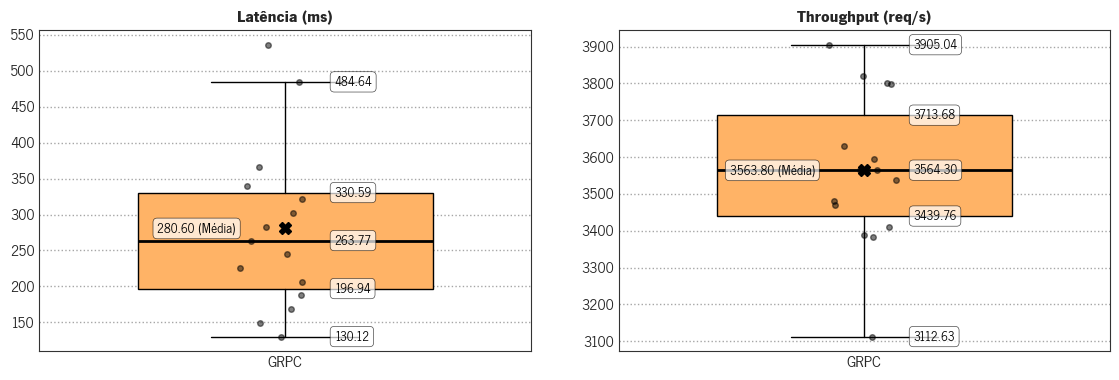
\includegraphics[width=1\linewidth]{imagens//resultados/5-resultados-simples-grpc-k6.png}
    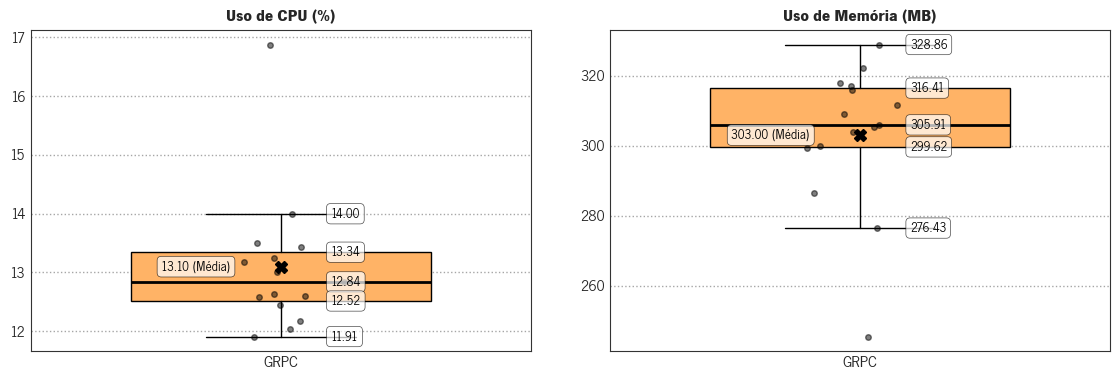
\includegraphics[width=1\linewidth]{imagens//resultados/5-resultados-simples-grpc-prometheus.png}    
    {\par \raggedright \footnotesize Fonte: Elaborado pelo autor.\par}
\end{figure}



\subsection{Thrift}

O Apache Thrift demonstrou desempenho intermediário no cenário simples, com tempo médio de resposta de 345,87 ms, aproximadamente \textbf{23\%} superior ao \gls{grpc}, como se observa na \autoref{tab:5-res-simples}. O tempo máximo registrado foi de 545,47ms, próximo ao observado no \gls{grpc}, sugerindo comportamento similar nos picos de latência. Os percentis de cauda apresentaram valores relevantes, com p90 de 401,14 ms e p95 de 435,93 ms, indicando uma distribuição de latência mais concentrada na faixa inferior em comparação ao tempo máximo. O throughput obtido foi de 2.891,20 req/s, posicionando-se entre o \gls{grpc} e o \gls{rest}.

\begin{table}[H]
\centering
\caption{Thrift comparado com os demais protocolos — Cenário Simples (\acrshort{grpc}/\gls{rest} em $\Delta$\% vs Thrift)}
\label{tab:5-res-simples-thrift}
\begin{tabular}[\linewidth]{lrrrrrrr}
\hline
Protocolo & Avg (ms) & Max (ms) & p90 (ms) & p95 (ms) & Throughput (req/s) & CPU (\%) & \acrshort{ram} (MB) \\
\hline
\textbf{Thrift} & \inferior{\textbf{345,87}} & \inferior{\textbf{545,47}} & \superior{\textbf{401,14}} & \superior{\textbf{435,93}} & \inferior{\textbf{2.891,20}} & \inferior{\textbf{14,00}} & \inferior{\textbf{315}} \\
\textbf{\acrshort{grpc}}   & \superior{-18,87\%} & \superior{-1,66\%} & \inferior{+9,02\%}  & \inferior{+14,74\%} & \superior{+23,26\%} & \superior{-6,43\%} & \superior{-3,81\%} \\
\textbf{\gls{rest}}   & \inferior{+37,99\%} & \inferior{+19,74\%} & \inferior{+27,25\%} & \inferior{+17,58\%} & \inferior{-27,53\%} & \inferior{+29,29\%} & \inferior{+14,92\%} \\
\hline
\end{tabular}
{\par \raggedright \footnotesize Fonte: Elaborado pelo autor.\par}
\end{table}

As amostras individuais do Thrift, conforme observado na \autoref{tab:5-res-simples-thrift} e ilustrado na \autoref{fig:5-simples-Thrift-k6}, revelaram consistência adequada caracterizada por latência média de 345,87 ms com desvio padrão reduzido (28,62 ms), enquanto os percentis de cauda (p90 = 401,14 ms; p95 = 435,93 ms) ficaram próximos ao máximo observado (545,47 ms), indicando baixa dispersão e ausência de outliers extremos. O comportamento observado sugere que a arquitetura do Thrift, com sua serialização binária proprietária que minimiza overhead de parsing e protocolo de transporte TCP direto que garante entrega ordenada com mínimo reenvio, oferece eficiência satisfatória para cenários simples. A diferença de desempenho em relação ao \gls{grpc} pode ser atribuída às otimizações específicas do \acrshort{http}/2, como a multiplexação de streams e cabeçalhos compactados, além da maturidade das implementações de Protocol Buffers, que conferem vantagem técnica ao \gls{grpc} em cenários de comunicação inter-serviços.

O uso de recursos do servidor pelo Thrift mostrou-se ligeiramente superior ao \gls{grpc}, com 14,00\% de utilização de CPU e 315MB de consumo de memória. Embora ainda em patamares baixos, esses valores indicam um overhead discreto em relação ao \gls{grpc}. A diferença na utilização de CPU pode relacionar-se às características específicas da serialização binária do Thrift e ao gerenciamento de conexões TCP, que podem demandar processamento adicional em comparação às otimizações nativas do \acrshort{http}/2.

\begin{figure}[H]
    \caption{Thrift: Dados de Execução (amostragem 15 execuções)}
    \label{fig:5-simples-Thrift-k6}
    \centering
    \includegraphics[width=1\linewidth]{imagens//resultados/5-resultados-simples-Thrift-k6.png}
    \includegraphics[width=1\linewidth]{imagens//resultados/5-resultados-simples-Thrift-prometheus.png}    
    {\par \raggedright \footnotesize Fonte: Elaborado pelo autor.\par}
\end{figure}



\subsection{\gls{rest}}

O protocolo \gls{rest} apresentou o menor desempenho no cenário simples, com tempo médio de resposta de 477,25ms (detalhes na \autoref{tab:5-res-simples-rest}), representando um overhead de aproximadamente \textbf{70\%} em relação ao \gls{grpc}. O tempo máximo observado foi de \textbf{653,16ms}, o mais elevado entre os três protocolos, indicando maior variabilidade de desempenho. Os percentis de cauda confirmam essa tendência, com p90 de \textbf{510,44ms} e p95 de \textbf{512,62ms}, demonstrando distribuição de latência mais concentrada, porém em patamares superiores. O throughput alcançado foi de \textbf{2.095,30 req/s}, o menor entre os protocolos testados.


\begin{table}[H]
\centering
\caption{\gls{rest} comparado com os demais protocolos — Cenário Simples (\acrshort{grpc}/Thrift em \Delta\% vs \gls{rest})}
\label{tab:5-res-simples-rest}
\begin{tabular}[\linewidth]{lrrrrrrr}
\hline
Protocolo & Avg (ms) & Max (ms) & p90 (ms) & p95 (ms) & Throughput (req/s) & CPU (\%) & \acrshort{ram} (MB) \\
\hline
\textbf{\gls{rest}}   & \inferior{\textbf{477,25}} & \inferior{\textbf{653,16}} & \inferior{\textbf{510,44}} & \inferior{\textbf{512,56}} & \inferior{\textbf{2.095,30}} & \inferior{\textbf{18,10}} & \inferior{\textbf{362}} \\
\textbf{\acrshort{grpc}}   & \superior{-41,20\%} & \superior{-17,87\%} & \superior{-14,32\%} & \superior{-2,42\%}  & \superior{+70,09\%} & \superior{-27,62\%} & \superior{-16,30\%} \\
\textbf{Thrift} & \superior{-27,53\%} & \superior{-16,49\%} & \superior{-21,41\%} & \superior{-14,95\%} & \superior{+37,99\%} & \superior{-22,65\%} & \superior{-12,98\%} \\
\hline
\end{tabular}
{\par \raggedright \footnotesize Fonte: Elaborado pelo autor.\par}
\end{table}

O consumo de recursos do servidor pelo \gls{rest}, conforme observamos na \autoref{fig:5-res-simples-rest} foi o mais elevado no cenário simples, com \textbf{18,10\%} de utilização de CPU e \textbf{362MB} de consumo de memória. Esses valores refletem o overhead inerente ao processamento de \acrshort{json} e às características do protocolo \acrshort{http}/1.1. A maior utilização de CPU indica que a serialização e desserialização de texto exigem mais ciclos de processamento em comparação aos formatos binários, enquanto o maior consumo de memória pode estar relacionado ao armazenamento temporário de strings \acrshort{json} e buffers de rede menos otimizados.

A análise das execuções individuais do \gls{rest}, conforme detalhado na \autoref{tab:5-res-simples-rest} e ilustrado na \autoref{fig:5-res-simples-rest}, revela comportamento previsível, com desempenho consistentemente inferior aos protocolos binários. Apesar da performance inferior, o \gls{rest} mantém uma estabilidade adequada, com tempos mantendo uma variação mínima e quantidade de throughput acima dos dois mil por segundo, confirmando sua viabilidade para cenários em que se prioriza a simplicidade de implementação e a interoperabilidade em detrimento da eficiência de comunicação. O comportamento observado alinha-se com as expectativas teóricas sobre protocolos baseados em texto versus protocolos binários em cenários de comunicação inter-serviços.

\begin{figure}[H]
    \caption{Rest: Dados de Execução (amostragem 15 execuções)}
    \label{fig:5-res-simples-rest}
    \centering
    \includegraphics[width=1\linewidth]{imagens//resultados/5-resultados-simples-Rest-k6.png}
    \includegraphics[width=1\linewidth]{imagens//resultados/5-resultados-simples-Rest-prometheus.png}    
    {\par \raggedright \footnotesize Fonte: Elaborado pelo autor.\par}
\end{figure}



\section{Cenário Tradicional}

Como descrito no \autoref{ch:4metodologia}, o cenário tradicional representa consultas de complexidade intermediária, exigindo processamento mais intensivo pelo módulo de \acrfull{ia} e maior troca de dados entre os microsserviços. As 15 execuções realizadas para cada protocolo revelam comportamentos distintos em condições de demanda moderada, em que tanto o processamento computacional quanto a comunicação inter-serviços contribuem significativamente para o tempo total de resposta. Analisando os dados detalhados na \autoref{tab:5-res-tradicioanl} e ilustrados comparativamente na \autoref{fig:5-res-tradicioanl}, observa-se, do lado do cliente, um aumento considerável nos tempos de resposta e a correspondente redução no \textit{throughput}. Do lado do servidor, o consumo de recursos cresce substancialmente, refletindo a maior demanda computacional do processamento de \gls{ia}.

\begin{figure}[H]
    \caption{Resultados Comparativos - Cenário Tradicional}
    \label{fig:5-res-tradicioanl}
    \centering
    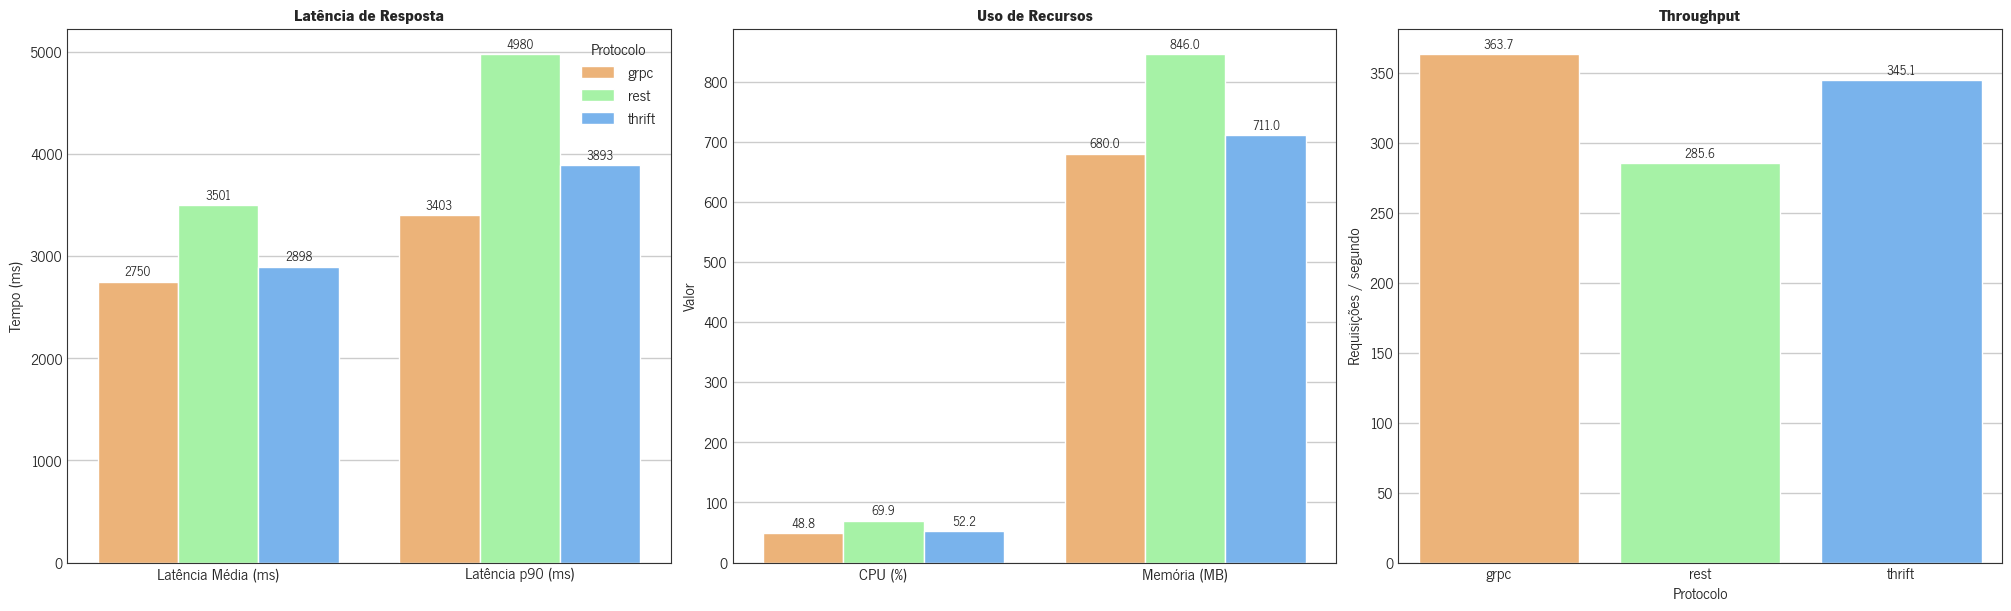
\includegraphics[width=1\linewidth]{imagens/resultados/5-resultados-tradicional.png}    
    {\par \raggedright \footnotesize Fonte: Elaborado pelo autor.\par}
\end{figure}


\begin{table}[H]
\centering
\caption{Métricas de desempenho e uso de recursos - Cenário Tradicional}
\label{tab:5-res-tradicioanl}
\begin{tabular}[\linewidth]{lrrrrrrr}
\hline
Protocolo & Avg (ms) & Max (ms) & p90 (ms) & p95 (ms) & Throughput (req/s) & CPU (\%) & \acrshort{ram} (MB) \\
\hline
\textbf{\acrshort{grpc}}   & 2.749,80 & 3.440,36 & 3.396,90 & 3.401,73 & 363,70 & 48,80 & 680 \\
\textbf{Thrift} & 2.897,87 & 3.969,82 & 3.892,62 & 3.923,65 & 345,10 & 52,20 & 711 \\
\textbf{\gls{rest}}   & 3.501,06 & 5.372,78 & 4.980,34 & 5.175,86 & 285,60 & 69,90 & 846 \\
\hline
\end{tabular}
{\par \raggedright \footnotesize Fonte: Elaborado pelo autor.\par}
\end{table}

\subsection{\acrshort{grpc}}

No cenário tradicional, o \gls{grpc} manteve sua posição de liderança em desempenho, registrando tempo médio de resposta de 2.749,80ms. O tempo máximo observado foi de 3.440,36ms, demonstrando que mesmo sob carga moderada, o protocolo mantém variabilidade controlada. Os percentis de cauda evidenciam comportamento robusto, com p90 de 3.396,90ms e p95 de 3.401,73ms, indicando distribuição de latência concentrada próxima ao valor máximo. O throughput foi de 363,70 req/s, uma redução significativa em relação ao cenário simples, mas ainda superior aos demais protocolos.

\begin{table}[H]
\centering
\caption{\gls{grpc} comparado com os demais protocolos — Cenário Tradicional (Thrift/\gls{rest} em $\Delta$\% vs \gls{grpc})}
\label{tab:5-res-tradicional-grpc}
\makebox[\textwidth][c]{%
\begin{tabular}{lrrrrrrr}
\hline
Protocolo & Avg (ms) & Max (ms) & p90 (ms) & p95 (ms) & Throughput (req/s) & CPU (\%) & \acrshort{ram} (MB) \\
\hline
\textbf{\acrshort{grpc}}   & \superior{\textbf{2.749,80}} & \superior{\textbf{3.440,36}} & \superior{\textbf{3.396,90}} & \superior{\textbf{3.401,73}} & \superior{\textbf{363,70}} & \superior{\textbf{48,80}} & \superior{\textbf{680}} \\
\textbf{Thrift} & \inferior{+5,40\%}  & \inferior{+15,38\%} & \inferior{+14,58\%} & \inferior{+15,35\%} & \inferior{-5,10\%}  & \inferior{+6,97\%}  & \inferior{+4,56\%} \\
\textbf{\gls{rest}}   & \inferior{+27,29\%} & \inferior{+56,15\%} & \inferior{+46,64\%} & \inferior{+52,19\%} & \inferior{-21,45\%} & \inferior{+43,23\%} & \inferior{+24,41\%} \\
\hline
\end{tabular}%
}
{\par \raggedright \footnotesize Fonte: Elaborado pelo autor.\par}
\end{table}


As execuções individuais, conforme apresentado na \autoref{tab:5-res-tradicional-grpc} e visualizado na \autoref{fig:5-Tradicional-gRPC-k6}, revelam que o \gls{grpc} escalou de forma linear e previsível em relação ao cenário simples, mantendo a eficiência de comunicação mesmo com payloads maiores e processamento mais intensivo. A diferença entre o tempo médio e os percentis de cauda sugere que o protocolo consegue absorver adequadamente os picos de processamento sem degradação significativa da performance. Essa característica é fundamental em aplicações financeiras, onde a consistência de resposta é tão importante quanto a velocidade absoluta, especialmente durante períodos de maior demanda computacional.

\begin{figure}[H]
    \caption{\acrshort{grpc}: Dados de Execução no Cenário Tradicional (amostragem 15 execuções)}
    \label{fig:5-Tradicional-gRPC-k6}
    \centering
    \includegraphics[width=1\linewidth]{imagens//resultados/5-resultados-Tradicional-gRPC-k6.png}
    \includegraphics[width=1\linewidth]{imagens//resultados/5-resultados-Tradicional-gRPC-prometheus.png}    
    {\par \raggedright \footnotesize Fonte: Elaborado pelo autor.\par}
\end{figure}


O uso de recursos do servidor aumentou substancialmente em relação ao cenário anterior, com 48,80\% de utilização de CPU e 680 MB de consumo de memória. Esses valores refletem a maior demanda computacional do processamento de \gls{ia}, mas ainda demonstram eficiência relativa do \gls{grpc}. A utilização de CPU próxima de 50\% indica que o sistema está operando em uma faixa adequada, com margem para picos de demanda, enquanto o consumo de memória duplicou em relação ao cenário simples, comportamento esperado devido ao maior volume de dados processados, os dados das execuções. Detalhes de todas as execuções podem ser vistas na  \autoref{fig:5-Tradicional-gRPC-k6}.

\subsection{Thrift}

O Apache Thrift apresentou tempo médio de resposta de 2.897,87ms no cenário tradicional, mantendo uma diferença de aproximadamente 5\% em relação ao \gls{grpc}. O tempo máximo registrado foi de 3.969,82ms, superior ao \gls{grpc}, indicando maior sensibilidade a picos de processamento. Os percentis de cauda mostram p90 de 3.892,62ms e p95 de 3.923,65ms, evidenciando distribuição de latência mais dispersa. O throughput foi de 345,10 req/s, ligeiramente inferior ao \gls{grpc}.

\begin{table}[H]
\centering
\caption{Thrift comparado com os demais protocolos — Cenário Tradicional (\acrshort{grpc}/\gls{rest} em $\Delta$\% vs Thrift)}
\label{tab:5-res-tradicional-thrift}
\makebox[\textwidth][c]{%
\begin{tabular}{lrrrrrrr}
\hline
Protocolo & Avg (ms) & Max (ms) & p90 (ms) & p95 (ms) & Throughput (req/s) & CPU (\%) & \acrshort{ram} (MB) \\
\hline
\textbf{Thrift} & \textbf{2.897,87} & \textbf{3.969,82} & \textbf{3.892,62} & \textbf{3.923,65} & \textbf{345,10} & \textbf{52,20} & \textbf{711} \\
\textbf{\acrshort{grpc}}   & \superior{-5,10\%}  & \superior{-13,36\%} & \superior{-12,73\%} & \superior{-13,30\%} & \superior{+5,39\%} & \superior{-6,51\%} & \superior{-4,36\%} \\
\textbf{\gls{rest}}   & \inferior{+20,83\%} & \inferior{+35,34\%} & \inferior{+27,93\%} & \inferior{+31,86\%} & \inferior{-17,23\%} & \inferior{+33,91\%} & \inferior{+19,01\%} \\
\hline
\end{tabular}%
}
{\par \raggedright \footnotesize Fonte: Elaborado pelo autor.\par}
\end{table}

A análise das amostras individuais do Thrift, conforme detalhado na \autoref{tab:5-res-tradicional-thrift} e visualizado na \autoref{fig:5-Tradicional-Thrift-k6}, revela comportamento estável, porém apresenta maior variabilidade em comparação ao \gls{grpc}. O protocolo demonstra escalabilidade adequada, mas evidencia sensibilidade superior às variações na carga de processamento. A diferença pronunciada nos valores máximos e percentis superiores sugere que o Thrift pode ser mais suscetível a gargalos em cenários de processamento intensivo, possivelmente relacionados a suas estratégias de buffering e ao gerenciamento das conexões \acrshort{tcp}.

\begin{figure}[H]
    \caption{Thrift: Dados de Execução no Cenário Tradicional (amostragem 15 execuções)}
    \label{fig:5-Tradicional-Thrift-k6}
    \centering
    \includegraphics[width=1\linewidth]{imagens//resultados/5-resultados-Tradicional-Thrift-k6.png}
    \includegraphics[width=1\linewidth]{imagens//resultados/5-resultados-Tradicional-Thrift-prometheus.png}    
    {\par \raggedright \footnotesize Fonte: Elaborado pelo autor.\par}
\end{figure}

O consumo de recursos do servidor apresentou 52,20\% de utilização de CPU e 711 MB de consumo de memória. Comparado ao \gls{grpc}, o Thrift apresentou overhead adicional de aproximadamente 7\% na CPU e 4\% na memória, esse número continua a tendência observada no cenário simples. Essa diferença pode estar relacionada às características específicas do protocolo \acrshort{tcp} direto e às estratégias de serialização do Thrift, que podem exigir processamento adicional em cenários de maior complexidade computacional.

\subsection{\gls{rest}}

O protocolo \gls{rest} registrou um tempo médio de resposta de 3.501,06 ms no cenário tradicional, enquanto Thrift e \acrshort{grpc} apresentaram diferenças de -17,23\% e -21,46\%, respectivamente. O tempo máximo observado foi significativamente elevado, atingindo 5.372,78 ms, indicando maior variabilidade de desempenho. Os percentis de cauda confirmam essa tendência, com p90 de 4.980,34ms e p95 de 5.175,86ms. O throughput alcançou 285,60 req/s; embora tenha sido o menor valor, permaneceu muito próximo dos demais.

\begin{table}[H]
\centering
\caption{\gls{rest} comparado com os demais protocolos — Cenário Tradicional ($\Delta$\% vs \gls{rest})}
\label{tab:5-res-tradicional-rest}
\makebox[\textwidth][c]{%
\begin{tabular}{lrrrrrrr}
\hline
Protocolo & Avg (ms) & Max (ms) & p90 (ms) & p95 (ms) & Throughput (req/s) & CPU (\%) & \acrshort{ram} (MB) \\
\hline
\textbf{\gls{rest}}   & \inferior{\textbf{3.501,06}} & \inferior{\textbf{5.372,78}} & \inferior{\textbf{4.980,34}} & \inferior{\textbf{5.175,86}} & \inferior{\textbf{285,60}} & \inferior{\textbf{69,90}} & \inferior{\textbf{846}} \\
\textbf{\acrshort{grpc}}   & \superior{-21,46\%} & \superior{-35,97\%} & \superior{-31,79\%} & \superior{-34,26\%} & \superior{+27,35\%} & \superior{-30,19\%} & \superior{-19,62\%} \\
\textbf{Thrift} & \superior{-17,23\%} & \superior{-26,11\%} & \superior{-21,78\%} & \superior{-24,19\%} & \superior{+20,83\%} & \superior{-25,32\%} & \superior{-15,96\%} \\
\hline
\end{tabular}%
}
{\par \raggedright \footnotesize Fonte: Elaborado pelo autor.\par}
\end{table}

As execuções individuais do \gls{rest} evidenciam o impacto cumulativo do overhead de serialização \acrshort{json} e protocolo \acrshort{http}/1.1 em cenários de maior complexidade. A diferença mais acentuada entre o tempo médio e os valores de cauda, conforme apresentado na \autoref{tab:5-res-tradicional-rest} e visualizada detalhadamente na \autoref{fig:5-Tradicional-REST-k6}, sugere que o \gls{rest} é especialmente sensível a variações na carga de processamento e no tamanho dos payloads. Essa característica pode representar um desafio em aplicações financeiras que requerem previsibilidade de desempenho, especialmente durante períodos de alta demanda em que a latência de cauda pode impactar significativamente a experiência do usuário.

\begin{figure}[H]
    \caption{\gls{rest}: Dados de Execução no Cenário Tradicional (amostragem 15 execuções)}
    \label{fig:5-Tradicional-REST-k6}
    \centering
    \includegraphics[width=1\linewidth]{imagens//resultados/5-resultados-Tradicional-REST-k6.png}
    \includegraphics[width=1\linewidth]{imagens//resultados/5-resultados-Tradicional-REST-prometheus.png}    
    {\par \raggedright \footnotesize Fonte: Elaborado pelo autor.\par}
\end{figure}

O uso de recursos do servidor pelo \gls{rest} foi significativamente superior, com 69,90\% de utilização de CPU e 846MB de consumo de memória. O Thrift por exemplo, utilizou 25,32\% a menos de CPU total. A elevada utilização de CPU indica que o processamento de \acrshort{json} e as características do \acrshort{http}/1.1 se tornam gargalos significativos em cenários de maior complexidade, enquanto o maior consumo de memória reflete o overhead das estruturas de dados textuais.

\section{Cenário Complexo}

O cenário complexo é o teste de estresse mais rigoroso, envolvendo consultas que exigem processamento intensivo de dados históricos e síntese avançada de informações pelo módulo de \acrfull{ia}. As 15 execuções neste cenário destacam o desempenho dos protocolos sob condições próximas aos limites operacionais, testando tanto o processamento computacional quanto a eficiência de comunicação ao extremo. No lado do cliente, há uma convergência dos tempos de resposta em relação aos \textit{timeouts} configurados, enquanto no lado do servidor, o uso de recursos se aproxima da saturação, especialmente para os protocolos menos eficientes. No entanto, as discrepâncias na eficiência de recursos e no \textit{throughput} persistiram, conforme ilustrado na \autoref{fig:resultados_complexo} e na \autoref{tab:res_complexo}.



\begin{figure}[H]
    \caption{Resultados Comparativos - Cenário Complexo}
    \label{fig:resultados_complexo}
    \centering
    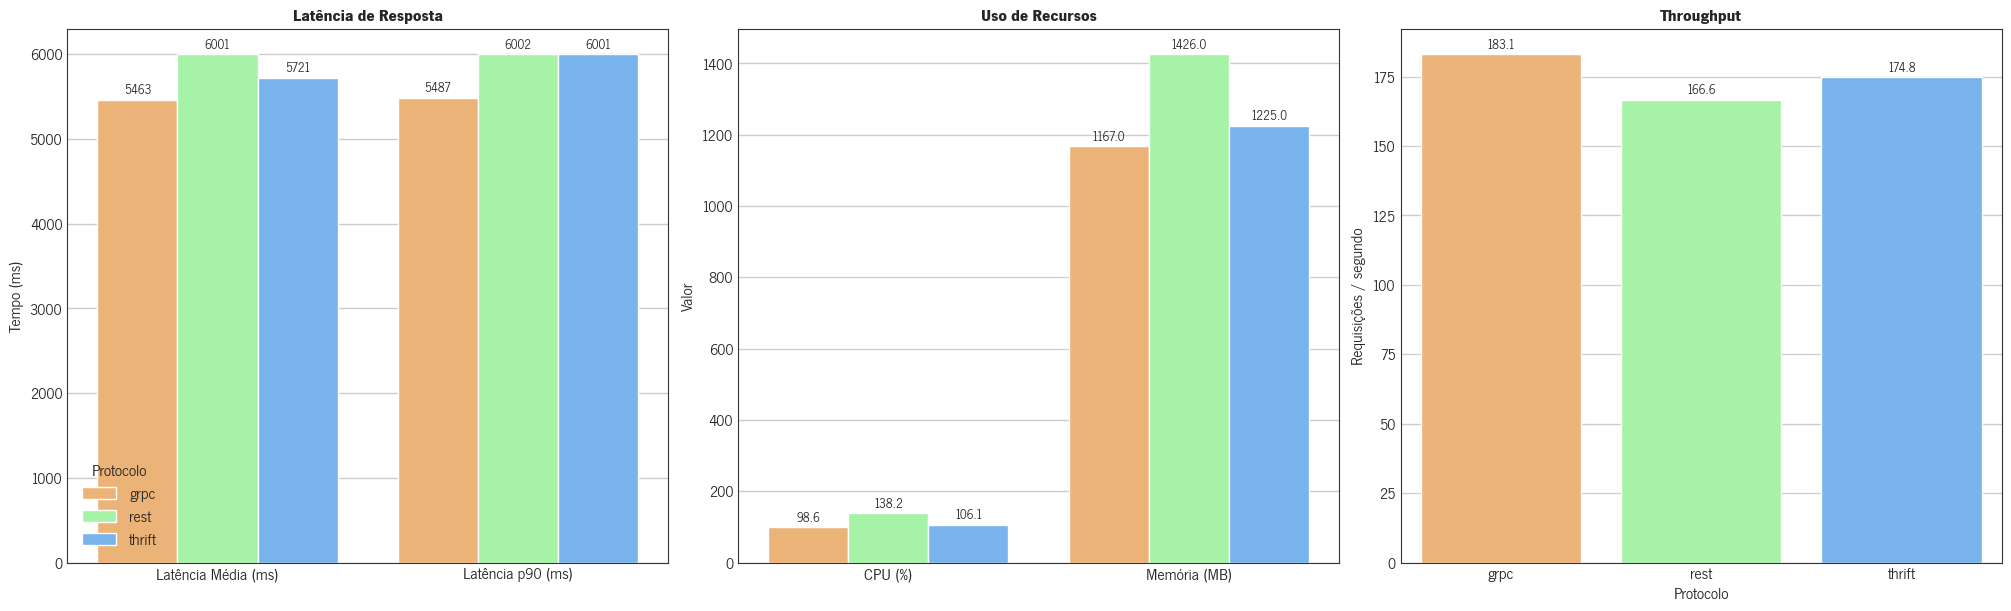
\includegraphics[width=1\linewidth]{imagens/resultados/5-resultados-complexo.png}    
    {\par \raggedright \footnotesize Fonte: Elaborado pelo autor.\par}
\end{figure}


\begin{table}[H]
\centering
\caption{Métricas de desempenho e uso de recursos - Cenário Complexo}
\label{tab:res_complexo}
\begin{tabular}[\linewidth]{lrrrrrrr}
\hline
Protocolo & Avg (ms) & Max (ms) & p90 (ms) & p95 (ms) & Throughput (req/s) & CPU (\%) & \acrshort{ram} (MB) \\
\hline
\textbf{\acrshort{grpc}}   & 5.462,68 & 5.499,37 & 5.486,74 & 5.490,84 & 183,10 & 98,60 & 1.167 \\
\textbf{Thrift} & 5.721,15 & 6.000,96 & 6.000,58 & 6.000,76 & 174,80 & 106,10 & 1.225 \\
\textbf{\gls{rest}}   & 6.000,97 & 6.002,16 & 6.001,80 & 6.001,84 & 166,60 & 138,20 & 1.426 \\
\hline
\end{tabular}
{\par \raggedright \footnotesize Fonte: Elaborado pelo autor.\par}
\end{table}

\subsection{\acrshort{grpc}}

No cenário complexo, o \gls{grpc} apresentou tempo médio de resposta de 5.462,68ms, mantendo sua eficiência relativa mesmo sob alta carga computacional. O tempo máximo observado foi de 5.499,37ms, demonstrando baixa variabilidade e comportamento altamente previsível. Os percentis de cauda evidenciam consistência excepcional, com p90 de 5.486,74ms e p95 de 5.490,84ms, valores muito próximos à média e ao máximo. O throughput foi de 183,10 req/s, ainda o melhor desempenho entre os protocolos testados (ver \autoref{tab:5-res-complexo-grpc}).

\begin{table}[H]
\centering
\caption{\gls{grpc} comparado com os demais protocolos — Cenário Complexo (Thrift/\gls{rest} em $\Delta$\% vs \gls{grpc})}
\label{tab:5-res-complexo-grpc}
\makebox[\textwidth][c]{%
\begin{tabular}{lrrrrrrr}
\hline
Protocolo & Avg (ms) & Max (ms) & p90 (ms) & p95 (ms) & Throughput (req/s) & CPU (\%) & \acrshort{ram} (MB) \\
\hline
\textbf{\acrshort{grpc}}   & \superior{\textbf{5.462,68}} & \superior{\textbf{5.499,37}} & \superior{\textbf{5.486,74}} & \superior{\textbf{5.490,84}} & \superior{\textbf{183,10}} & \superior{\textbf{98,60}} & \superior{\textbf{1.167}} \\
\textbf{Thrift} & \inferior{+4,73\%}  & \inferior{+9,14\%}  & \inferior{+9,35\%}  & \inferior{+9,30\%}  & \inferior{-4,53\%}  & \inferior{+7,61\%}  & \inferior{+4,97\%} \\
\textbf{\gls{rest}}   & \inferior{+9,87\%}  & \inferior{+9,14\%}  & \inferior{+9,38\%}  & \inferior{+9,32\%}  & \inferior{-9,02\%}  & \inferior{+40,21\%} & \inferior{+22,23\%} \\
\hline
\end{tabular}%
}
{\par \raggedright \footnotesize Fonte: Elaborado pelo autor.\par}
\end{table}

A análise das execuções individuais, conforme apresentado na \autoref{tab:5-res-complexo-grpc} e visualizado na \autoref{fig:5-Complexo-gRPC-k6}, revela que o \gls{grpc} manteve estabilidade notável mesmo no cenário mais exigente, com todas as amostras concentradas em uma faixa estreita de valores. Essa característica sugere que o protocolo consegue otimizar eficientemente a comunicação inter-serviços mesmo quando o processamento de \gls{ia} representa a maior parte do tempo de resposta. A baixa dispersão dos valores indica que o \gls{grpc} oferece previsibilidade superior em cenários críticos, aspecto fundamental para sistemas financeiros que operam com \acrshort{sla}s rigorosos e requerem comportamento determinístico.

\begin{figure}[H]
    \caption{\acrshort{grpc}: Dados de Execução no Cenário Complexo (amostragem 15 execuções)}
    \label{fig:5-Complexo-gRPC-k6}
    \centering
    \includegraphics[width=1\linewidth]{imagens//resultados/5-resultados-Complexo-gRPC-k6.png}
    \includegraphics[width=1\linewidth]{imagens//resultados/5-resultados-Complexo-gRPC-prometheus.png}    
    {\par \raggedright \footnotesize Fonte: Elaborado pelo autor.\par}
\end{figure}

O uso de recursos do servidor atingiu 98,60\% de utilização de CPU e 1.167MB de consumo de memória, indicando operação próxima aos limites, mas ainda de forma controlada. Mesmo sob alta carga, o \gls{grpc} conseguiu manter eficiência relativa, evitando saturação completa dos recursos. O consumo de memória, embora elevado, permaneceu em patamares gerenciáveis, variando entre 1.076 MB e 1.248 MB, demonstrando que o protocolo lida com grandes volumes de dados de forma otimizada.

\subsection{Thrift}

O Apache Thrift registrou tempo médio de resposta de 5.721,15ms no cenário complexo, representando um overhead de aproximadamente 5\% em relação ao \gls{grpc}. O tempo máximo observado foi de 6.000,96ms, coincidindo com os percentis de cauda que apresentaram p90 de 6.000,58ms e p95 de 6.000,76ms, todos próximos ao limite de \textit{timeout} configurado (conforme estruturado em \autoref{sec:5-metricas-variaveis}). O throughput foi de 174,80 req/s, inferior ao \gls{grpc} mas ainda competitivo.

\begin{table}[H]
\centering
\caption{Thrift comparado com os demais protocolos — Cenário Complexo (\acrshort{grpc}/\gls{rest} em $\Delta$\% vs Thrift)}
\label{tab:5-res-complexo-thrift}
\makebox[\textwidth][c]{%
\begin{tabular}{lrrrrrrr}
\hline
Protocolo & Avg (ms) & Max (ms) & p90 (ms) & p95 (ms) & Throughput (req/s) & CPU (\%) & \acrshort{ram} (MB) \\
\hline
\textbf{Thrift} & \textbf{5.721,15} & \textbf{6.000,96} & \textbf{6.000,58} & \textbf{6.000,76} & \textbf{174,80} & \textbf{106,10} & \textbf{1.225} \\
\textbf{\acrshort{grpc}}   & \superior{-4,52\%}  & \superior{-8,37\%}  & \superior{-8,54\%}  & \superior{-8,46\%}  & \superior{+4,75\%}  & \superior{-7,06\%}  & \superior{-4,74\%} \\
\textbf{\gls{rest}}   & \inferior{+4,90\%}  & \inferior{+0,20\%}  & \inferior{+0,02\%}  & \inferior{+0,02\%}  & \inferior{-4,69\%}  & \inferior{+30,27\%} & \inferior{+16,41\%} \\
\hline
\end{tabular}%
}
{\par \raggedright \footnotesize Fonte: Elaborado pelo autor.\par}
\end{table}

As amostras individuais do Thrift, conforme detalhado na \autoref{tab:5-res-complexo-thrift} e visualizado na \autoref{fig:5-Complexo-Thrift-k6}, revelam um padrão interessante, em que várias execuções atingiram valores próximos ao \textit{timeout} configurado, sugerindo que o protocolo aproximou-se de seus limites operacionais neste cenário. Essa característica indica que o Thrift, embora eficiente em cenários simples e tradicionais, pode enfrentar desafios em situações de extrema complexidade computacional. O comportamento observado sugere possível saturação das conexões \acrshort{tcp} ou limitações no gerenciamento de buffers durante processamento intensivo, aspectos que devem ser considerados em implementações de produção.

\begin{figure}[H]
    \caption{Thrift: Dados de Execução no Cenário Complexo (amostragem 15 execuções)}
    \label{fig:5-Complexo-Thrift-k6}
    \centering
    \includegraphics[width=1\linewidth]{imagens//resultados/5-resultados-Complexo-Thrift-k6.png}
    \includegraphics[width=1\linewidth]{imagens//resultados/5-resultados-Complexo-Thrift-prometheus.png}    
    {\par \raggedright \footnotesize Fonte: Elaborado pelo autor.\par}
\end{figure}


O consumo de recursos atingiu 106,10\% de utilização de CPU e 1.225MB de consumo de memória, indicando saturação dos recursos computacionais. A utilização de CPU superior a 100\% sugere que o sistema operou em condições de stress, possivelmente utilizando recursos de múltiplos cores de forma intensiva. O maior consumo de memória em relação ao \gls{grpc} pode estar relacionado a estratégias menos otimizadas de gerenciamento de buffers durante processamento intensivo.

\subsection{\gls{rest}}

O protocolo \gls{rest} apresentou tempo médio de resposta de 6.000,97 ms no cenário complexo, atingindo consistentemente valores próximos ao limite de \textit{timeout}. O tempo máximo registrado foi de 6.002,16 ms, com percentis p90 e p95 de 6.001,80 ms e 6.001,84 ms respectivamente, todos concentrados no limite superior configurado. O throughput foi de 166,60 req/s, o menor entre os três protocolos.

\begin{table}[H]
\centering
\caption{\gls{rest} comparado com os demais protocolos — Cenário Complexo (\acrshort{grpc}/Thrift em $\Delta$\% vs \gls{rest})}
\label{tab:5-res-complexo-rest}
\makebox[\textwidth][c]{%
\begin{tabular}{lrrrrrrr}
\hline
Protocolo & Avg (ms) & Max (ms) & p90 (ms) & p95 (ms) & Throughput (req/s) & CPU (\%) & \acrshort{ram} (MB) \\
\hline
\textbf{\gls{rest}}   & \inferior{\textbf{6.000,97}} & \inferior{\textbf{6.002,16}} & \inferior{\textbf{6.001,80}} & \inferior{\textbf{6.001,84}} & \inferior{\textbf{166,60}} & \inferior{\textbf{138,20}} & \inferior{\textbf{1.426}} \\
\textbf{\acrshort{grpc}}   & \superior{-8,96\%}  & \superior{-8,37\%}  & \superior{-8,55\%}  & \superior{-8,51\%}  & \superior{+9,90\%}  & \superior{-28,67\%} & \superior{-18,19\%} \\
\textbf{Thrift} & \superior{-4,66\%}  & \superior{-0,02\%}  & \superior{-0,02\%}  & \superior{-0,02\%}  & \superior{+4,92\%}  & \superior{-23,25\%} & \superior{-14,11\%} \\
\hline
\end{tabular}%
}
{\par \raggedright \footnotesize Fonte: Elaborado pelo autor.\par}
\end{table}

A análise das execuções do \gls{rest}, conforme apresentado na \autoref{tab:5-res-complexo-rest} e visualizado na \autoref{fig:5-Complexo-REST-k6}, no cenário complexo revela que o protocolo atingiu sistematicamente seus limites operacionais, com praticamente todas as amostras próximas ao \textit{timeout} configurado. Esse comportamento indica que o overhead cumulativo da serialização \acrshort{json} e do protocolo \acrshort{http}/1.1 se torna crítico em cenários de alta complexidade computacional. Os resultados sugerem que o \gls{rest} pode não ser adequado para aplicações que requerem processamento intensivo de \gls{ia} em tempo real, especialmente quando múltiplos microsserviços precisam trocar grandes volumes de dados de forma eficiente.

\begin{figure}[H]
    \caption{\gls{rest}: Dados de Execução no Cenário Complexo (amostragem 15 execuções)}
    \label{fig:5-Complexo-REST-k6}
    \centering
    \includegraphics[width=1\linewidth]{imagens//resultados/5-resultados-Complexo-REST-k6.png}
    \includegraphics[width=1\linewidth]{imagens//resultados/5-resultados-Complexo-REST-prometheus.png}    
    {\par \raggedright \footnotesize Fonte: Elaborado pelo autor.\par}
\end{figure}


O uso de recursos do servidor foi o mais elevado, com 138,20\% de utilização de CPU e 1.426MB de consumo de memória, indicando saturação completa do sistema. A utilização de CPU muito superior a 100\% demonstra que o protocolo \gls{rest} exigiu recursos computacionais além da capacidade disponível, resultando em degradação significativa de performance. O maior consumo de memória entre todos os protocolos reflete o overhead das estruturas de dados textuais e o gerenciamento menos eficiente de buffers em condições extremas.

\section{Análise Geral}

A análise comparativa dos três cenários, conforme observada detalhadamente na \autoref{tab:res_todos_agrupados}, revela padrões consistentes de desempenho que se alinham com as características técnicas fundamentais de cada protocolo. O \gls{grpc} demonstrou superioridade em todos os cenários, mantendo os menores tempos médios de resposta, maior throughput e menor variabilidade, evidenciada por valores próximos entre média, percentis de cauda e máximos. Essa característica de previsibilidade é particularmente valiosa em sistemas financeiros, onde \acrshort{sla}s rigorosos demandam comportamento determinístico. Em termos de recursos, o \gls{grpc} manteve o menor consumo de CPU e memória em todos os cenários, evidenciando eficiência operacional superior. O Thrift apresentou desempenho intermediário satisfatório nos cenários simples e tradicional, mas evidenciou limitações significativas no cenário complexo, onde a utilização de CPU ultrapassou 100\%, indicando saturação dos recursos. O \gls{rest}, embora funcional em todos os cenários, demonstrou degradação progressiva de desempenho, culminando em saturação sistemática no cenário complexo com 138\% de utilização de CPU.

\begin{table}[H]
\centering
\caption{Métricas (média e p95) por cenário e protocolo}
\label{tab:res_todos_agrupados},
\setlength{\tabcolsep}{4pt}
\renewcommand{\arraystretch}{1.15}
\begin{tabularx}{\linewidth}{l X | r | r | r | r | r | r | r | r |}
\hline
\multicolumn{2}{c}{} & \multicolumn{2}{c}{\textbf{Latência (ms)}} & \multicolumn{2}{c}{\textbf{Vazão (req/s)}} & \multicolumn{2}{c}{\textbf{CPU (\%)}} & \multicolumn{2}{c}{\textbf{\acrshort{ram} (MB)}} \\
\cline{3-10}
\textbf{Cenário} & \textbf{Prot.} & Avg & p95 & Avg & p95 & Avg & p95 & Avg & p95 \\
\hline
\multirow{3}{*}{Simples}
  & \textbf{\acrshort{grpc}}   & 280,60   & 500,18   & 3.563,80 & 3.845,10 & 13,10  & 14,86  & 303   & 324  \\
  & \textbf{Thrift} & 345,87   & 457,20   & 2.891,20 & 3.156,78 & 14,00  & 15,48  & 315   & 343  \\
  & \textbf{\gls{rest}}   & 477,25   & 614,30   & 2.095,30 & 2.459,30 & 18,10  & 19,29  & 362   & 406  \\
\hline
\multirow{3}{*}{Tradicional}
  & \textbf{\acrshort{grpc}}   & 2.749,80 & 3.422,25 & 363,70   & 409,20   & 48,80  & 53,54  & 680   & 744  \\
  & \textbf{Thrift} & 2.897,87 & 3.923,65 & 345,10   & 387,94   & 52,20  & 58,31  & 711   & 771  \\
  & \textbf{\gls{rest}}   & 3.501,06 & 5.175,86 & 285,60   & 312,42   & 69,90  & 76,81  & 846   & 910  \\
\hline
\multirow{3}{*}{Complexo}
  & \textbf{\acrshort{grpc}}   & 5.462,68 & 5.490,84 & 183,10   & 195,59   & 98,60  & 106,27 & 1.167 & 1.279 \\
  & \textbf{Thrift} & 5.721,15 & 6.000,76 & 174,80   & 186,69   & 106,10 & 117,91 & 1.225 & 1.340 \\
  & \textbf{\gls{rest}}   & 6.000,97 & 6.002,01 & 166,60   & 180,61   & 138,20 & 159,71 & 1.426 & 1.502 \\
\hline
\end{tabularx}
{\par \raggedright \footnotesize Fonte: Elaborado pelo autor.\par}
\end{table}

Uma observação particularmente interessante emerge da análise dos valores máximos em relação às médias e do comportamento da utilização de recursos. Enquanto no cenário simples a diferença entre média e máximo foi significativa para todos os protocolos (91\% para \gls{grpc}, 58\% para Thrift, 37\% para \gls{rest}), no cenário complexo essa diferença praticamente desapareceu, indicando que o processamento intensivo de \gls{ia} tende a homogeneizar os tempos de resposta. Paralelamente, observou-se que a utilização de CPU cresceu de forma não linear: no cenário simples, todos os protocolos operaram abaixo de 20\% de CPU; no tradicional, entre 49\% e 70\%, e no complexo, entre 99\% e 138\%. O consumo de memória, por outro lado, apresentou crescimento mais linear, variando de aproximadamente 300MB no cenário simples para 1.400MB no complexo, sugerindo que o gargalo principal está no processamento computacional, não no armazenamento de dados.

Os resultados obtidos corroboram os achados de \textcite{niswar_performance_2024}, descritos no \autoref{ch:3estado_da_arte}, essas vantagens tornaram-se ainda mais pronunciadas em cenários de alta complexidade computacional. Os conceitos abordados nos pilares teóricos sobre escalabilidade e observabilidade manifestam-se claramente nos dados, onde a capacidade do \gls{grpc} de manter latência de cauda previsível e menor consumo de recursos reflete diretamente em maior facilidade de monitoramento e definição de \acrshort{sla}s. A convergência dos protocolos no cenário complexo ilustra o princípio da orquestração eficiente discutido no referencial teórico, em que a escolha do protocolo de comunicação pode determinar a viabilidade de sistemas distribuídos em cargas extremas, aspecto fundamental para a resiliência operacional no setor financeiro, onde a eficiência de recursos impacta diretamente os custos operacionais e a capacidade de escalar sob demanda. A convergência dos protocolos no cenário complexo também ilustra o princípio da orquestração eficiente discutido no referencial teórico, onde a escolha do protocolo de comunicação pode determinar a viabilidade de sistemas distribuídos em cargas extremas, aspecto fundamental para a resiliência operacional no setor financeiro, onde a eficiência de recursos diretamente impacta os custos operacionais e a capacidade de escalar sob demanda.